\documentclass[aspectratio=169]{beamer}
\setbeamertemplate{navigation symbols}{}
\usepackage{color,amsmath,comment, subfigure}
\usepackage{booktabs}
\usepackage{url}

%\setbeameroption{show notes}

%%%%%%%%%%%%%%%%%%%%%%%%%%
\title[]{Class 8: Spread of disease in networks}
\author[]{Matthew J. Salganik}
\institute[]{Sociology 204: Social Networks, Spring 2021\\Princeton University}
\date[]{
3/3: Large scale sexual network in Likoma, Malawi
\vfill 

\begin{flushleft}
\vspace{0.6in}

\includegraphics[width=0.1\textwidth]{figures/cc.png}
\end{flushleft}

}

\note{
TODO: Move candy bowl to the end of this class possibly. Helps set the stage for next class and has them do it before they see the readings
TODO: Try to find movie of chains of affection
}

\begin{document}
%%%%%%%%%%%%%%%%%%%%%%%%%%%
\frame{\titlepage}
%%%%%%%%%%%%%%%%%%%%%%%%%%%
\begin{frame}
\frametitle{}

\begin{center}
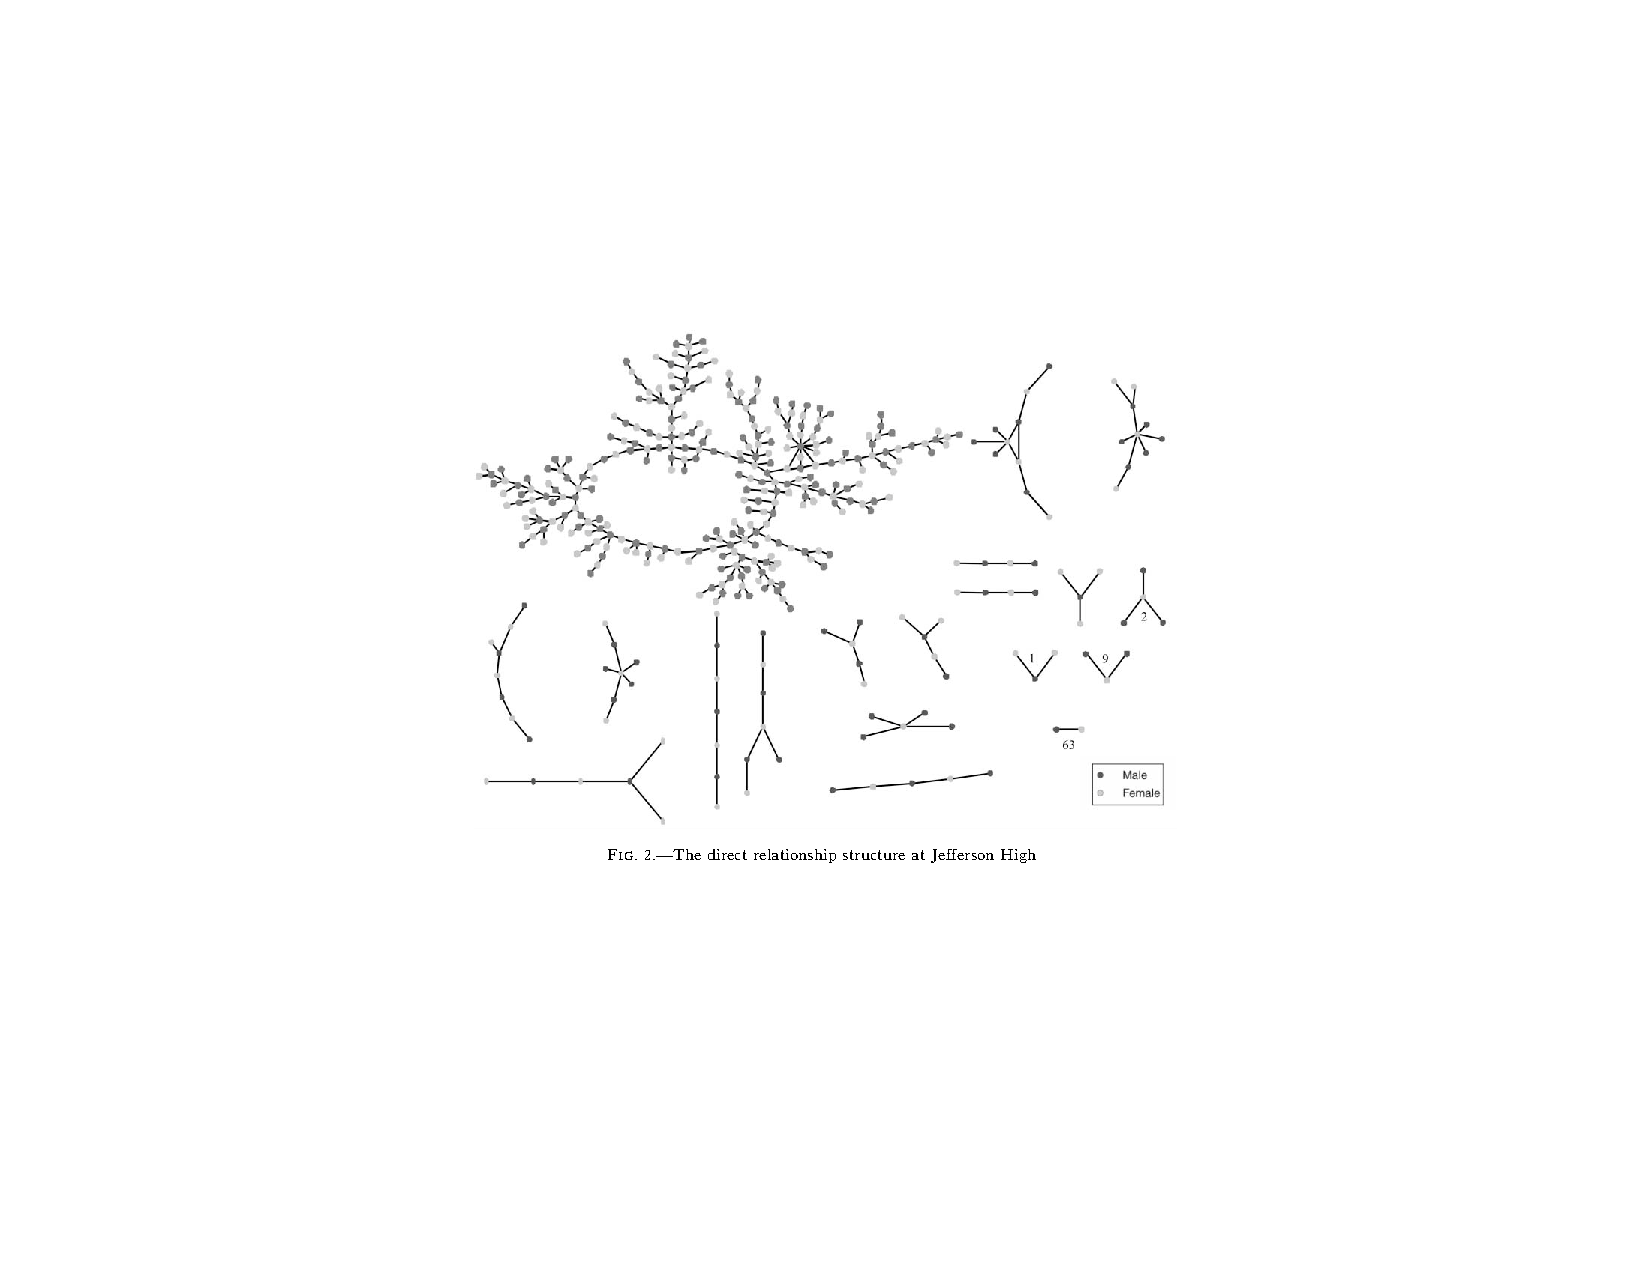
\includegraphics[width = 0.80\textwidth]{figures/bearman_chains_2004_fig2}
\end{center}

\note{

}


\end{frame}
%%%%%%%%%%%%%%%%%%%%%%%%%%%%%%%%%%
\begin{frame}

\begin{center}

\includegraphics[width= 0.95\textwidth]{figures/helleringer_sexual_2007_title}
\end{center}

\tiny{\url{http://www.ncbi.nlm.nih.gov/pubmed/18090281}}

\note{

Bearman et al. studies a school in the US.  Helleringer et al are interested in sub-Saharan Africa.  About two-thirds of the worlds HIV cases are in sub-Saharan Africa and patterns of infection are different there than in other countries.  UNAIDS divides countries into no epidemic, concentrated epidemic, and generalized epidemic.  Malawi has a generalized epidemic.  That is why information about the structure of the sexual network in the general population is so important.  Also, there is something of a puzzle about why HIV rates are so much higher in sub-Saharan Africa.  This is part of trying to figure that out.

Basically, the do a network census on an island (Fig.~\ref{fig:likoma_map}).  Like Bearman et al. they find one giant component but it includes more cycles than the spanning tree in the high school. (Figure~\ref{fig:helleringer_sexual_2007_fig2a}). 

}

\end{frame}
%%%%%%%%%%%%%%%%%%%%%%%%%%%
\begin{frame}

\begin{center}
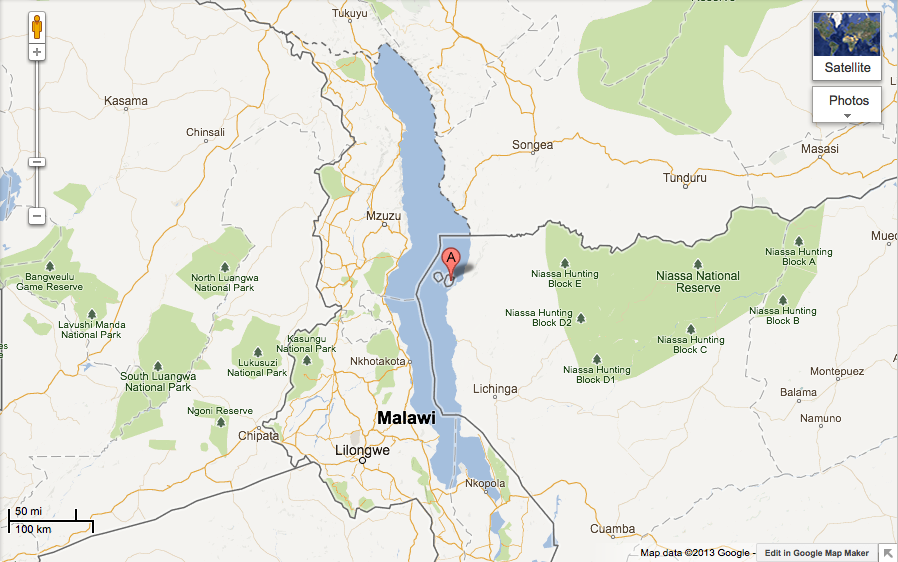
\includegraphics[width = 0.90\textwidth]{figures/likoma_map}
\end{center}

\end{frame}
%%%%%%%%%%%%%%%%%%%%%%%%%%%
\begin{frame}

\begin{center}
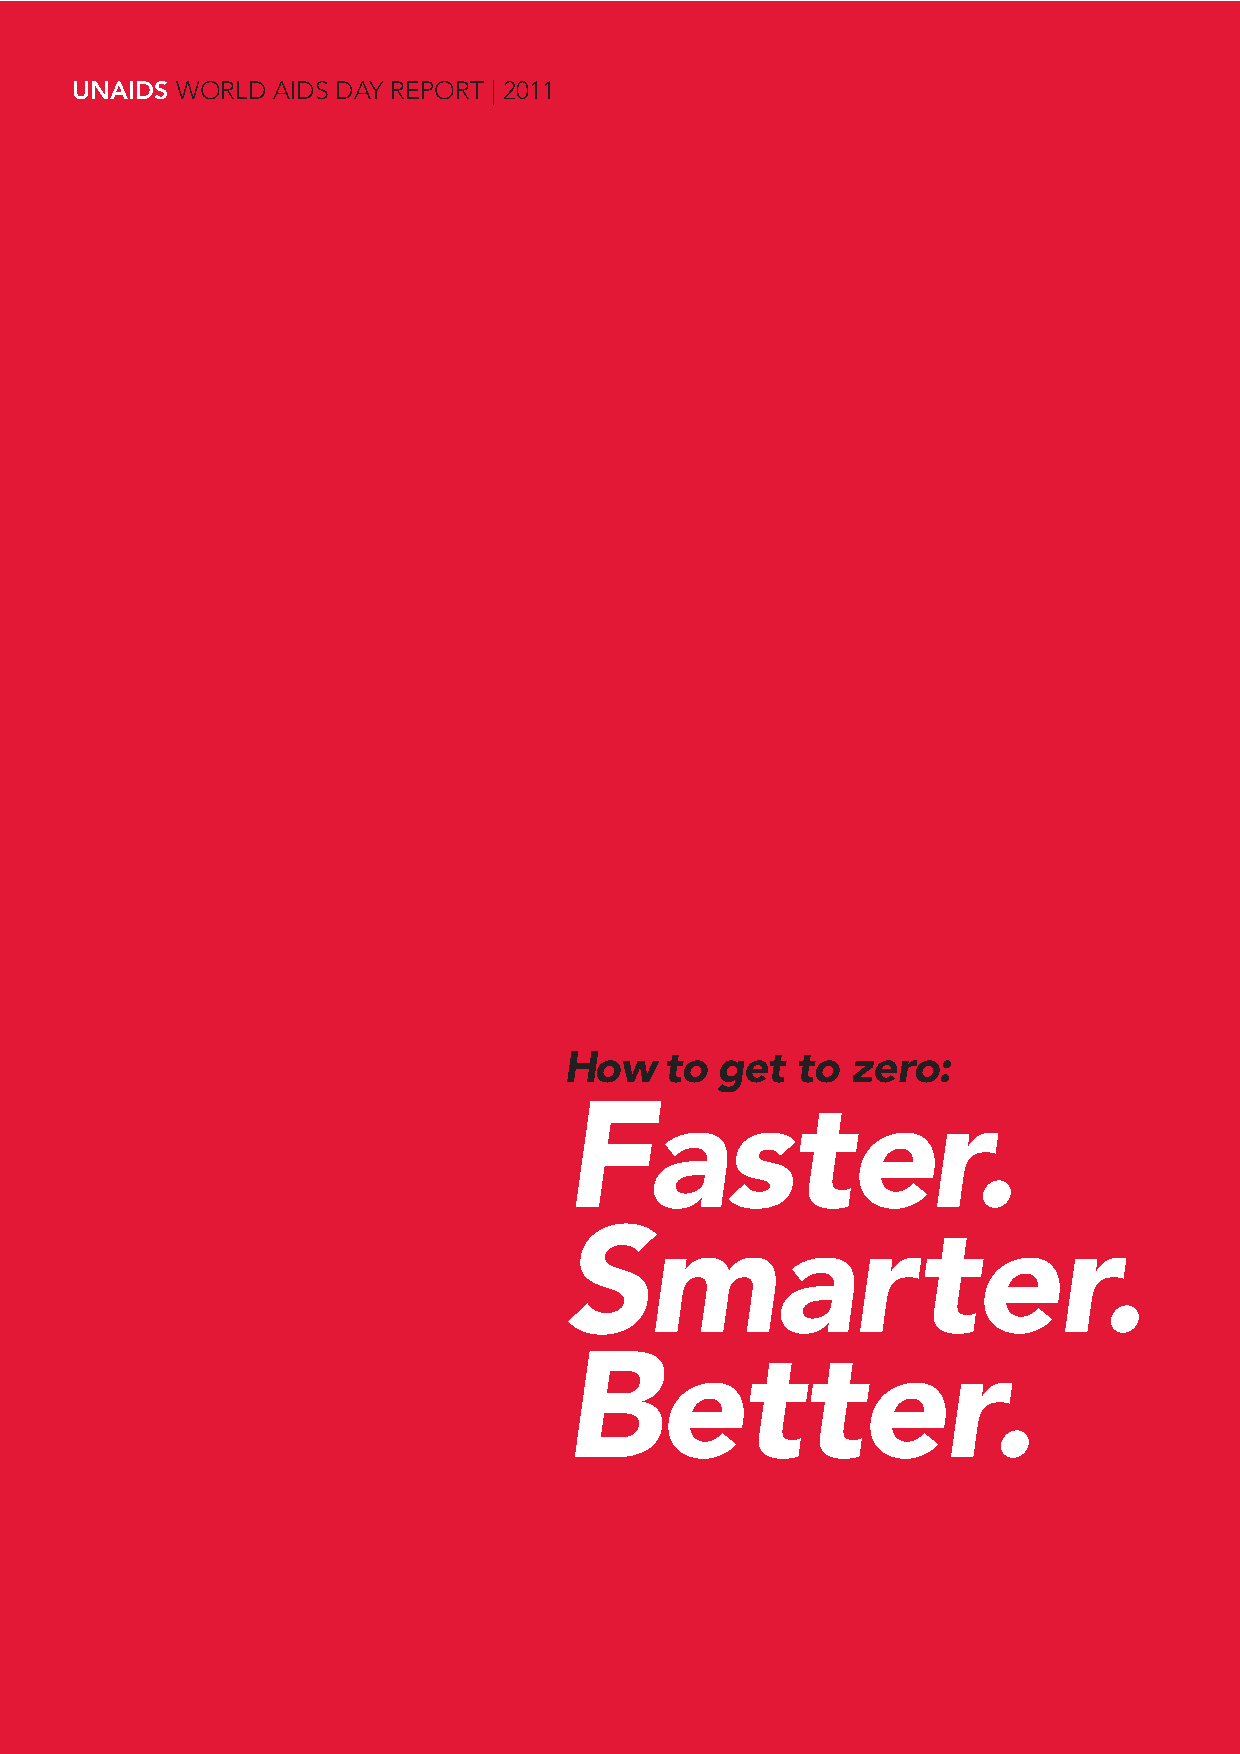
\includegraphics[height = 0.9\textheight]{figures/unaids_report_cover_2011}
\end{center}

\note{
we care because HIV prevalence higher in sub-Saharan Africa
}

\end{frame}
%%%%%%%%%%%%%%%%%%%%%%%%%%%
\begin{frame}

\begin{center}
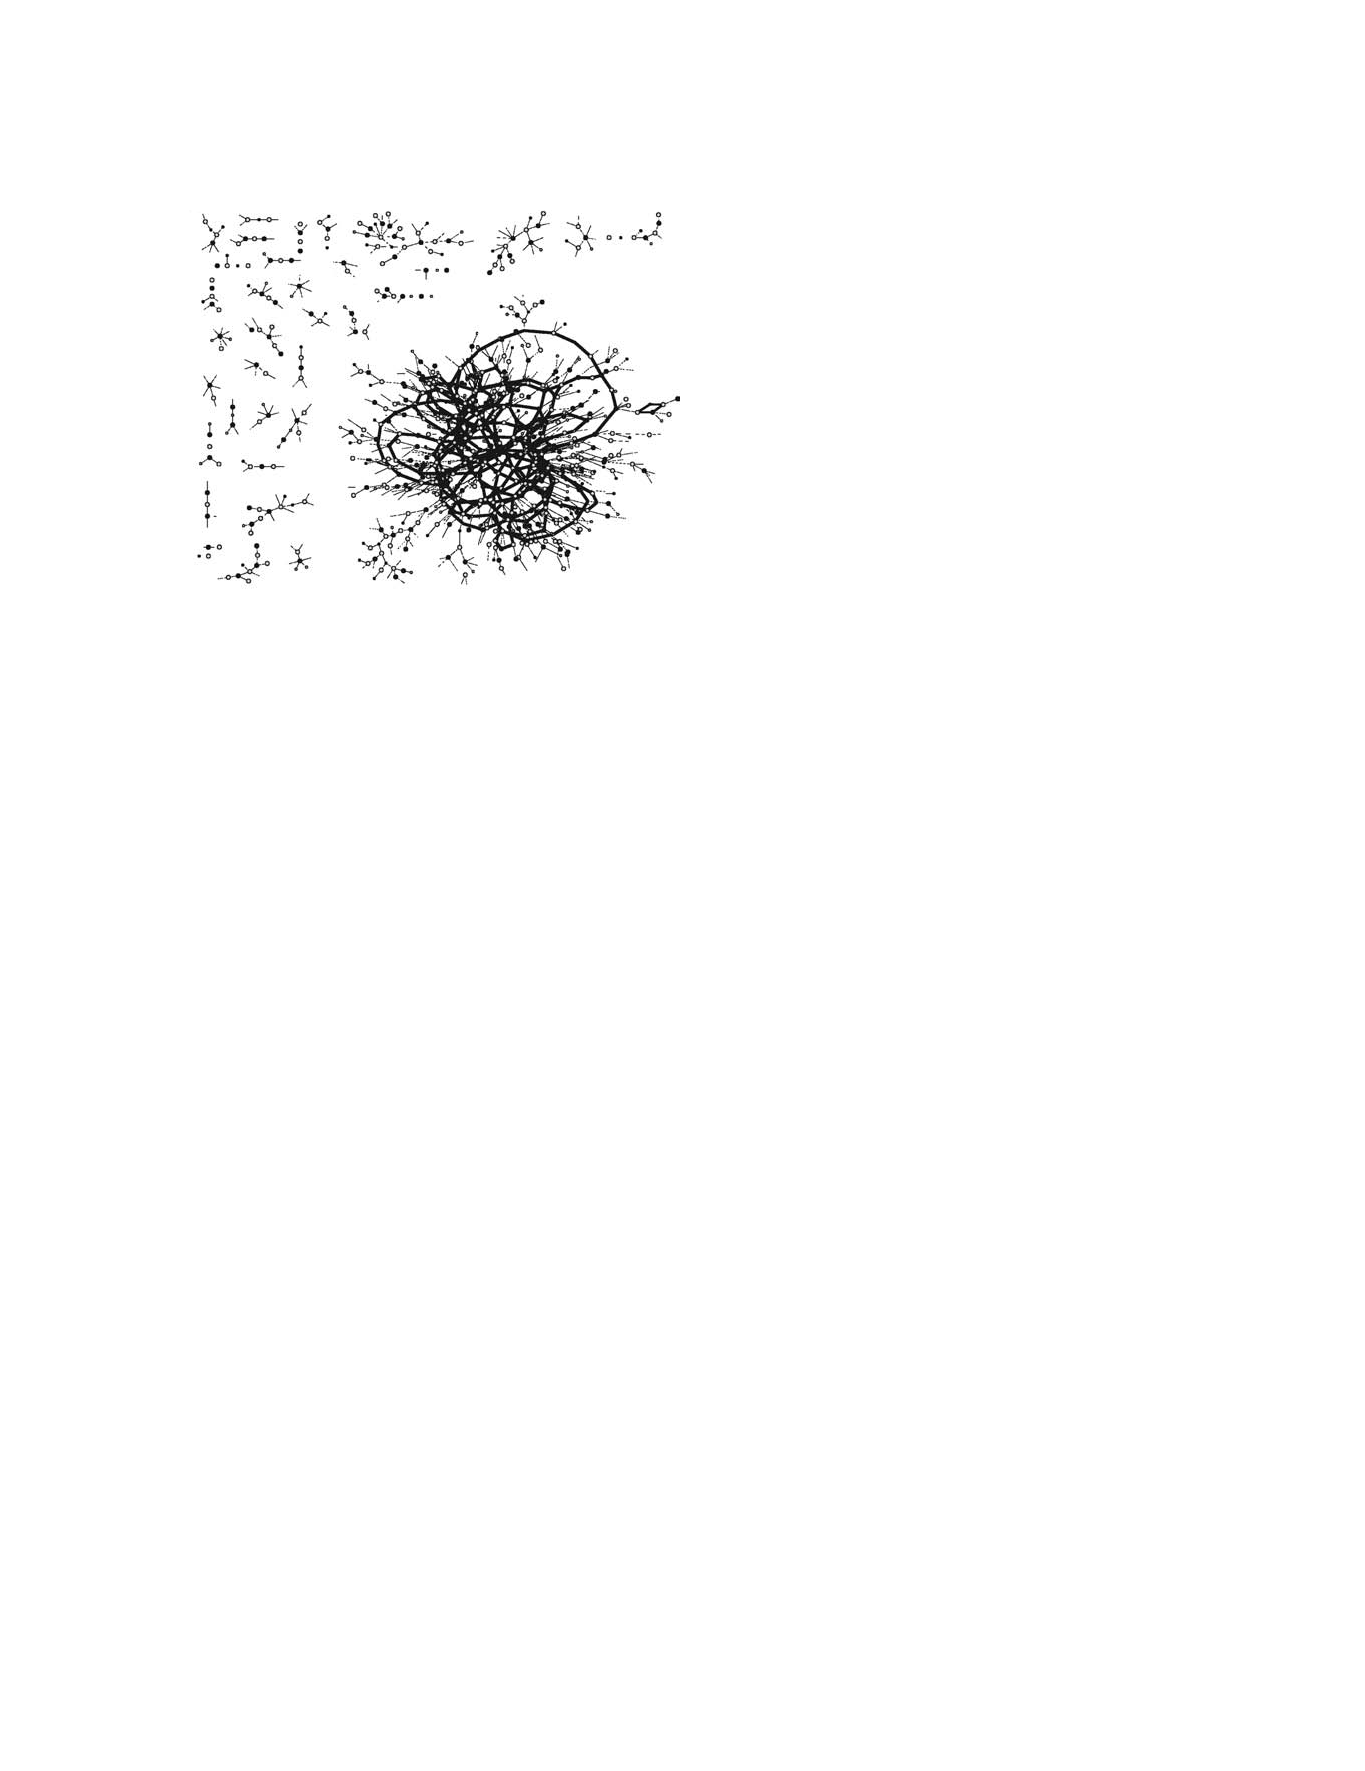
\includegraphics[height = 0.75\textheight]{figures/helleringer_sexual_2007_fig2a}
\end{center}

\vfill

Last 3 years

\note{

Full network 3 year recall period

darker lines represent cycles

}

\end{frame}
%%%%%%%%%%%%%%%%%%%%%%%%%%%
\begin{frame}
\frametitle{}

\begin{center}
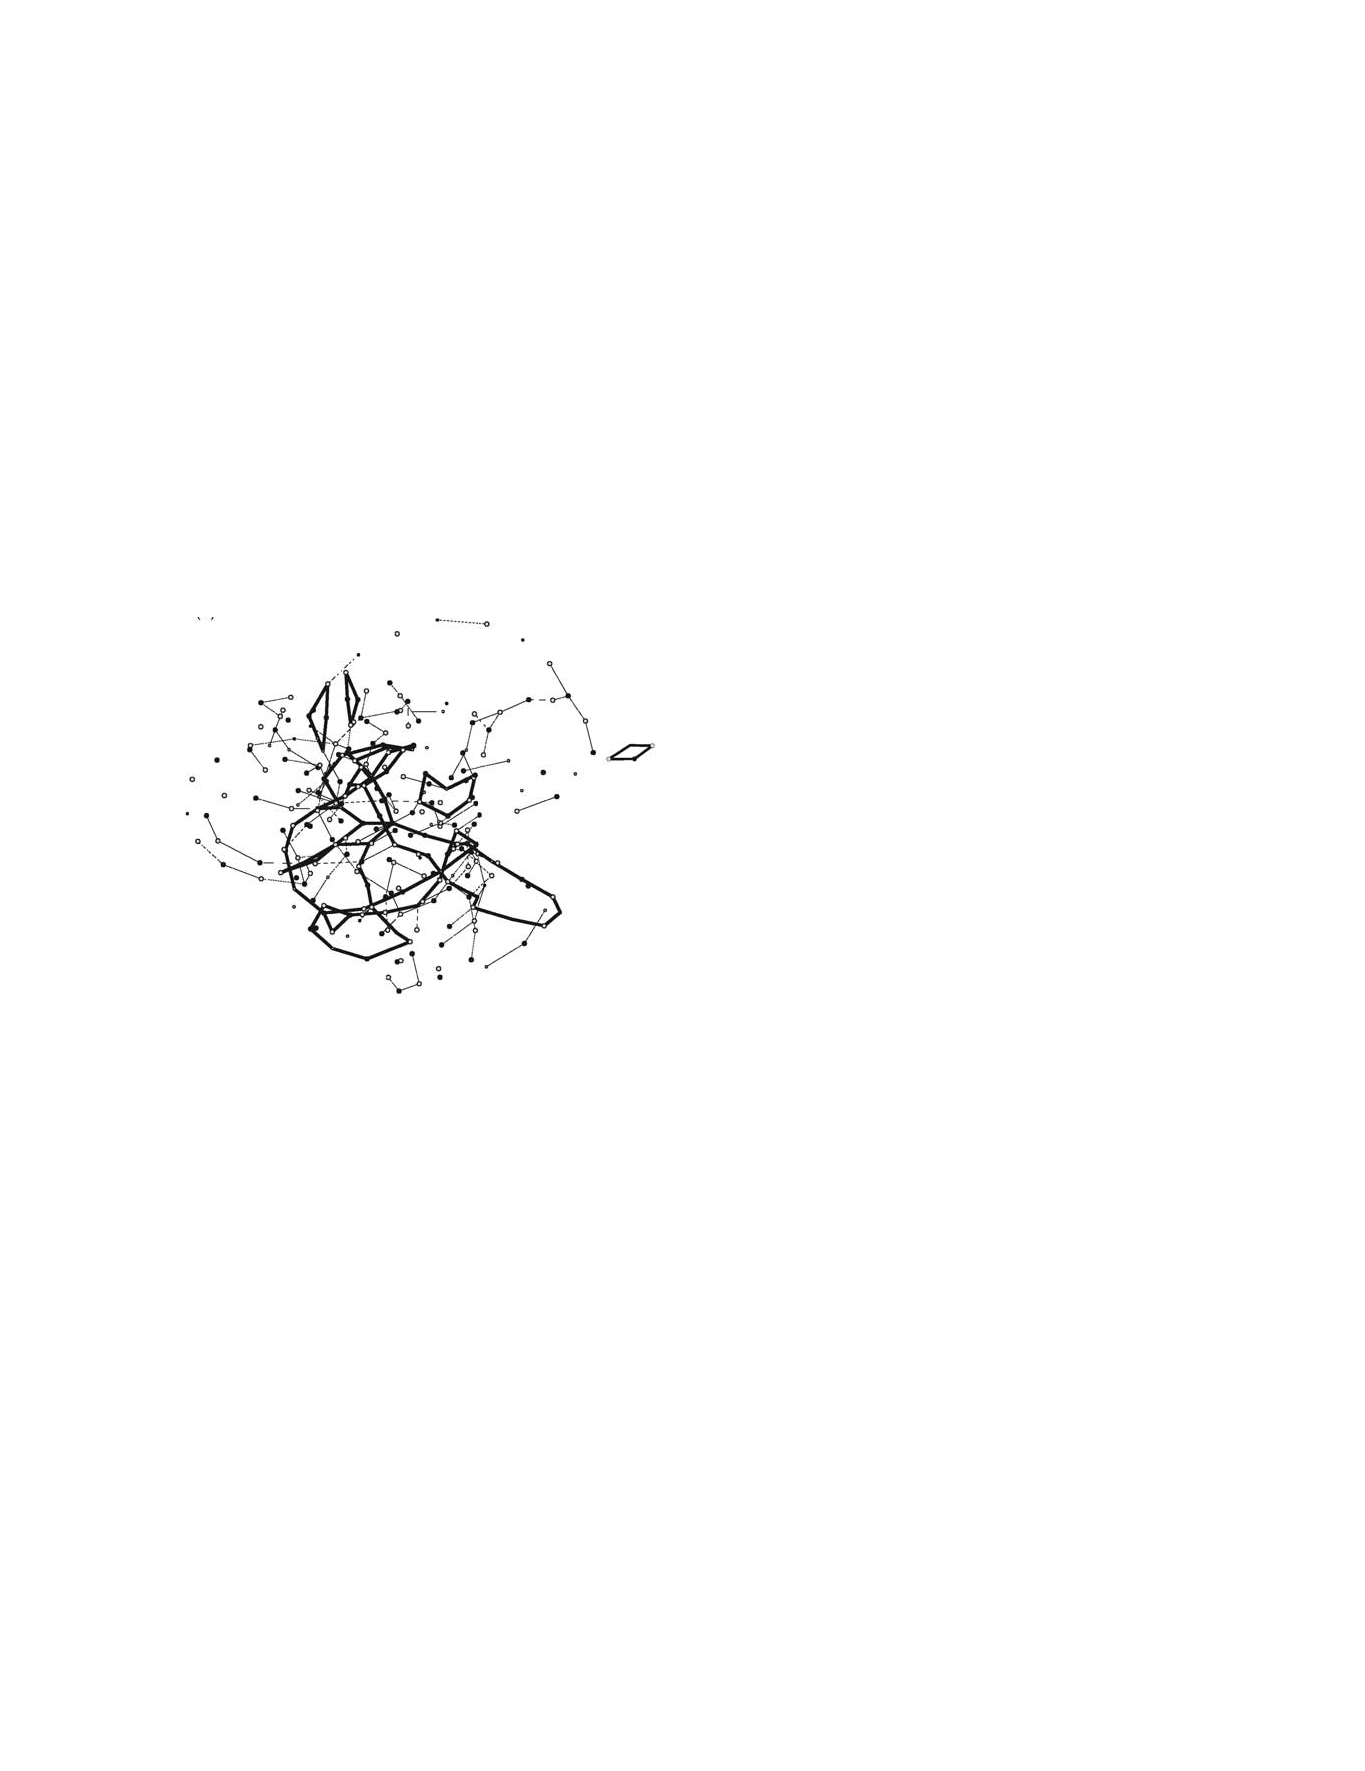
\includegraphics[height = 0.75\textheight]{figures/helleringer_sexual_2007_fig2b}
\end{center}

\vfill

Last year

\note{

last year

}

\end{frame}
%%%%%%%%%%%%%%%%%%%%%%%%%%%
\begin{frame}

\begin{center}
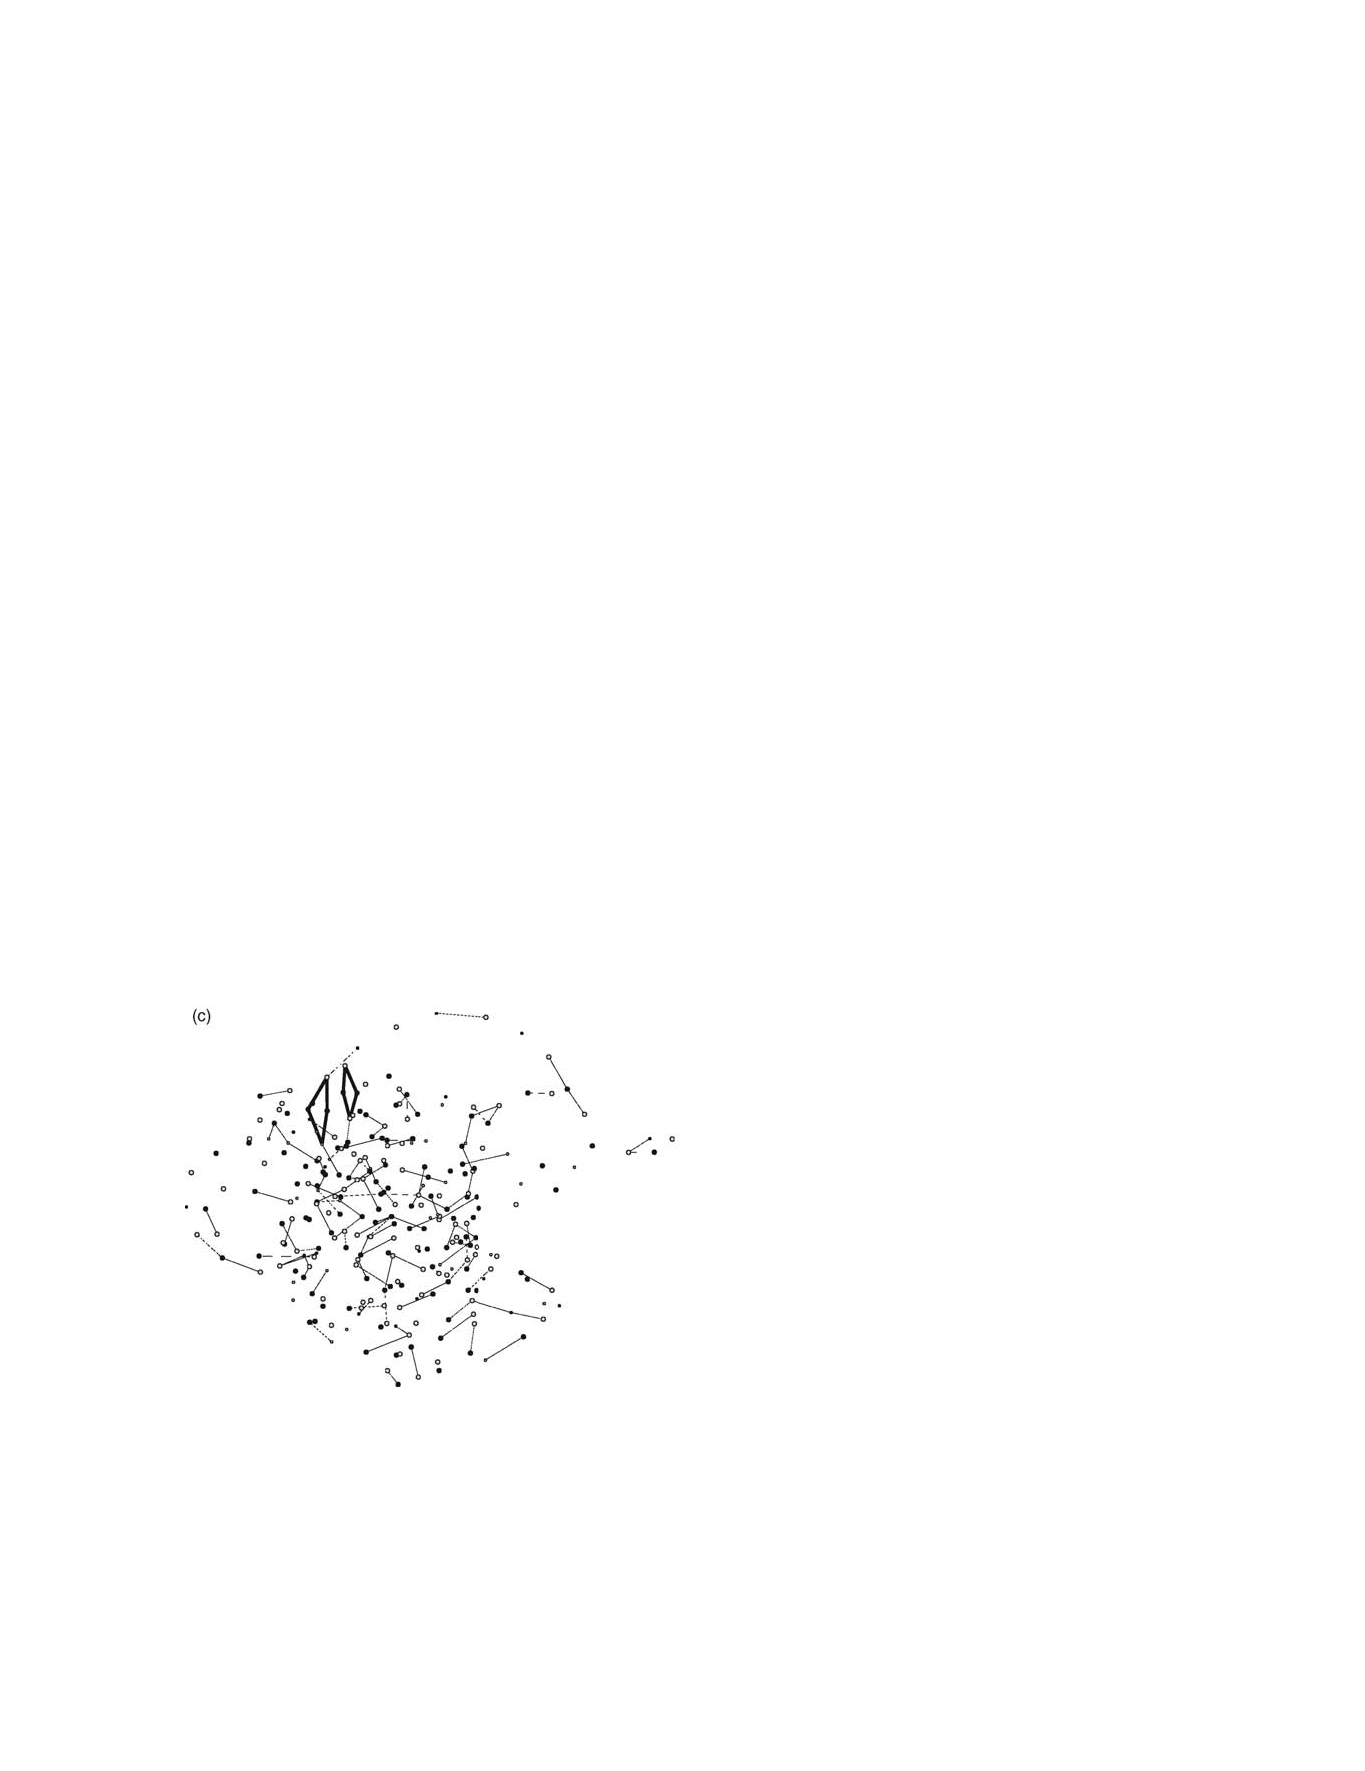
\includegraphics[height = 0.75\textheight]{figures/helleringer_sexual_2007_fig2c}
\end{center}

\vfill

Right now

\note{


note concurrency

}

\end{frame}
%%%%%%%%%%%%%%%%%%%%%%%%%%
\begin{frame}

\begin{center}
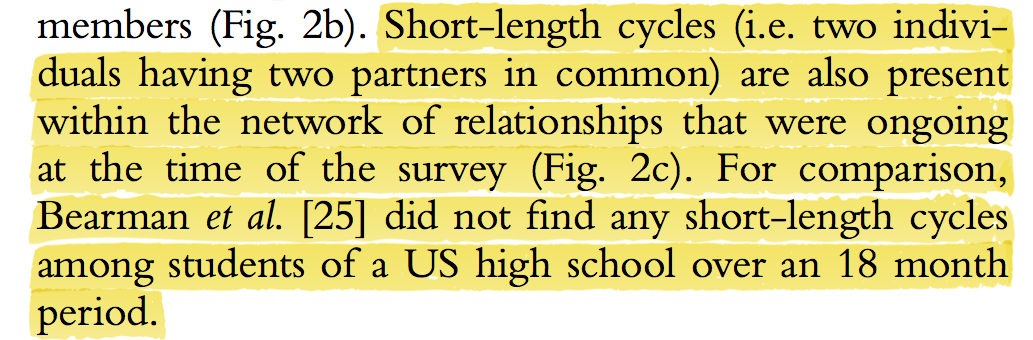
\includegraphics[width = 0.95\textwidth]{figures/helleringer_sexual_2007_cycles}
\end{center}

\note{
why the difference, we don't know.  Stephane wanted to collect another round of data but funding was cut
}

\end{frame}
%%%%%%%%%%%%%%%%%%%%%%%%%
\begin{frame}

Summary:
\begin{itemize}
\item contact patterns are important for the spread of disease
\pause
\item sometimes detailed complete network structure matters
\pause
\item simple rules by individuals can aggregate to complex network patterns
\end{itemize}

\end{frame}
%%%%%%%%%%%%%%%%%%%%%%%%%
\begin{frame}

Next class: Madness of Crowds
\begin{itemize}
\item Watts, Chapter 7.
\item Asch, S.E. (1955). Opinions and social pressure. \textit{Scientific American}, 193(5):31-35. (Available on Canvas)
\item Easley D. and Kleinberg, J. (2010). ``Networks, Crowds, and Markets: Chapter 16''. (skim mathematical model in Sections 16.3-16.6)
\item Tierney, J. (2007). Diet and fat: A severe case of mistaken consensus. \textit{New York Times}
\end{itemize}

\end{frame}
%%%%%%%%%%%%%%%%%%%%%%%%%%

\end{document}
